\documentclass[12pt]{article}


\usepackage{algorithmic} %Für Pseudocode https://math-linux.com/latex-26/faq/latex-faq/article/how-to-write-algorithm-and-pseudocode-in-latex-usepackage-algorithm-usepackage-algorithmic
\usepackage{stmaryrd} %Für Widerspruchsblitz
\usepackage{amsmath} 
\usepackage{amssymb}
\usepackage{amsthm} %Für Theoreme und Beweise
\usepackage{graphicx} %Für Bilder

\newtheoremstyle{break}% name
  {}%         Space above, empty = `usual value'
  {}%         Space below
  {\itshape}% Body font
  {}%         Indent amount (empty = no indent, \parindent = para indent)
  {\bfseries}% Thm head font
  {.}%        Punctuation after thm head
  {\newline}% Space after thm head: \newline = linebreak
  {}%         Thm head spec

\theoremstyle{break}

\renewcommand{\thesection}{\Roman{section}}
\renewcommand{\thesubsection}{\arabic{subsection}}

%Definiere Satz, Definition,...
\newtheorem{theorem}{Satz}[subsection]
\newtheorem{korollar}[theorem]{Korollar}
\newtheorem{definition}[theorem]{Definition}
\newtheorem{algorithm}[theorem]{Algorithmus}
\newtheorem{comment}[theorem]{Bemerkung}
\newtheorem{problem}[theorem]{Problem}
\newtheorem{example}[theorem]{Beispiel}
\newtheorem{nothing}[theorem]{}

\author{Prof. Schaedle}
\title{Numerik 1 (ohne Beweise)}

\begin{document}
\maketitle

\newpage

\section{Numerische Integration}

\subsection{Einführung}

\begin{problem}
Gegeben $f: [a,b] \rightarrow \mathbb{N}$ mit $a, b \in \mathbb{R}$.
Berechne $\int_a^b f(x) dx $
\end{problem}

\begin{example}
\begin{description}
  \item 
\end{description}
\begin{enumerate}
  \item Archimedes (282-212 v.Chr.): Fläche unter einer Parabel \\ \\
    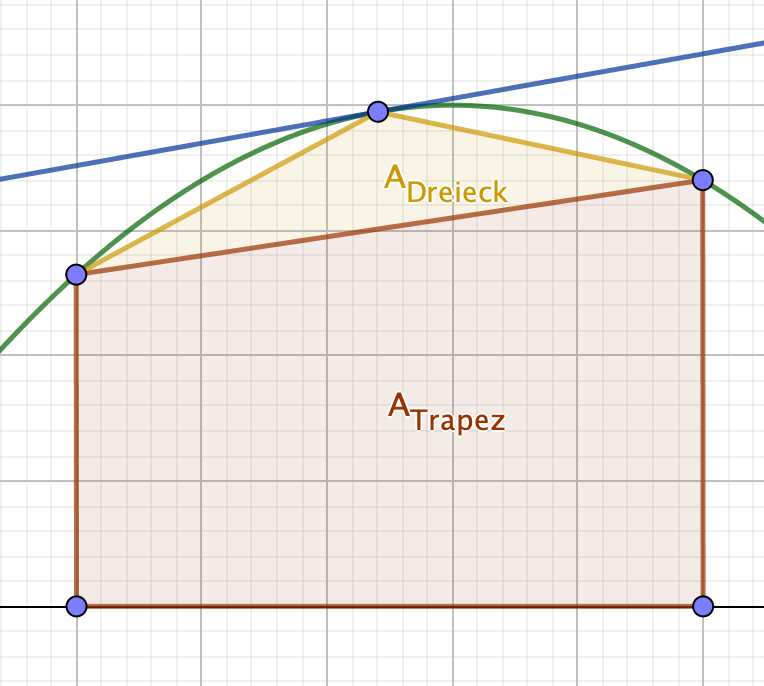
\includegraphics[width=5cm]{Kapitel_1/Grafiken/Grafik_1.png} \\
    $A_{Parabel} = A_{Trapez} + \frac{4}{3} A_{Dreieck}$
  \item Leibniz + Newton (~1670):
    $$ \int_a^b f(x) dx = F(b) - F(a),$$ wobei $\frac{d}{dx} F(x) = f(x)$
  \item Riemann (~1850): 
    $$ \int_a^b f(x) dx = \lim\limits_{\vert \Delta \vert \to \infty} \sum_{j=1}^n f(\xi_j)(x_j - x_{j-1}),$$
    wobei $\Delta = (x_0,...,x_n)$ Gitter Zerlegung von $[a, b]$, $a=x_0 < ...< x_n = b$, $\xi_j \in [x_{j-1}, x_j]$ und $\vert \Delta \vert := \max_{j=1,...n} \vert x_j - x_{j-1} \vert$.
    Das Riemannintegral existiert, falls: 
    $$ \forall \varepsilon > 0 \exists \delta > 0: \vert \Delta \vert < \delta \Rightarrow \vert \int_a^b f(X) dx - \sum_{j=1}^n f(\xi_j)(x_j-x_{j-1}) \vert < \varepsilon $$
\end{enumerate}
\end{example}

\begin{comment}[Approximation von Integralen]
\begin{description}
  \item 
\end{description}
\begin{enumerate}
  \item (linke) Rechtecksregel: 
    $$\int_{x_{j-1}}^{x_{j-1}+h} f(x) dx \approx h f(x_{j-1})$$
    $$\int_a^b f(x) dx = \sum_{j=1}^n \int_{x_{j-1}}^{x_j} f(x)dx \approx \sum_{j=1}^n f(x_{j-1}) (x_j-x_{j-1})$$
  \item Mittelpunktsregel:
    $$\int_{x_{j}}^{x_{j}+h} f(x) dx \approx f\left(\frac{x_j+x_j+h}{2}\right)h$$
    $$\int_a^bf(x)dx \approx \sum_{j=1}^n f\left( \frac{x_{j-1} + x_j}{2}\right) (x_j - x_{j-1})$$
    Da mit Hilfe der Transformationsformel sich jedes Integral $\int_{x_{j-1}}^{x_j}$ auf ein Integral $\int_a^b$ transformieren lässt, betrachten wir ohne Einschränkungen Integrale von $0$ bis $1$. Nutze dazu die Abb. $[a, b] \rightarrow [x_{j-1}, x_j], t \mapsto x_{j-1} + t(x_j - x_{j-1})$.
    $$ \int_{x_{j-1}}^{x_j} f(x) dx = \int_0^1 \underbrace{f\left( x_{j-1} + t(x_j - x_{j-1})\right)}_{:= g_{j-1}(t)} (x_j - x_{j-1})dt = \int_0^1 g_{j-1}(t)(x_j-x_{j-1})dt$$
\end{enumerate}
\end{comment}

\begin{definition}[Quadraturformel]
Eine s-stufige Quadraturformel zur Approximation von $\int_0^1 g(t)dt$ mit Knoten $c_i$ und Gewichten $b_i$ für $i=1,...s$ ist gegeben durch 
$$\sum_{i=1}^s b_i g(c_i) \left( \approx \int_0^1 g(t) dt\right)$$

\end{definition}

\begin{example}
\begin{description}
  \item 
\end{description}
\begin{enumerate}
  \item Rechtecksregel: $s = 1, b_1 = 1, c_1 = 0$
    $$ \int_0^1 g(t) \approx b_1 g(c_1) = g(0)$$
  \item Mittelpunktsregel: $s = 1, b_1 = 1, c_1 = \frac{1}{2}$
    $$ \int_0^1 g(t) \approx g\left(\frac{1}{2}\right)$$
  \item Trapezregel: $s=2, b_1=b_2= \frac{1}{2}, c_1 = 0, c_2 = 1$
    $$ \int_0^1 g(t) \approx \frac{1}{2} g(0) + \frac{1}{2}g(1)$$
  \item Simpsonregel: $s=3, b_1 =  \frac{1}{6}, b_2 =  \frac{2}{3}, b_3 =  \frac{1}{6}, c_1 = 0, c_2 =  \frac{1}{2}, c_3 = 1$
    $$ \int_0^1 g(t) \approx \frac{1}{6} \left(g(0) + 4g\left(\frac{1}{2}\right) +g(1)\right)$$ 
    \textbf{Herleitung:} Man legt eine Parabel $p$ durch die Punkte $(0, g(0)), (\frac{1}{2}, g(\frac{1}{2})), (1, g(1))$ und integriert $p$ von 0 bis 1. \\
    $p(t) = g(0)(1-t)2(\frac{1}{2}-t) + g(\frac{1}{2})(1-t)4t + g(1)(\frac{1}{2}-t)2t$ \\
    $$\Rightarrow \int_0^1 p(t)dt = \frac{1}{6}g(0)+ \frac{2}{3}g\left(\frac{1}{2}\right) +\frac{1}{6}g(1)$$ 
  \item "pulcherrima et utilissima regula" von Newton:
    $$\int_0^1 g(t) dt \approx \frac{1}{8}\left(g(0) + 3g\left(\frac{1}{3}\right) + 3g\left(\frac{2}{3}\right) + g(1)\right)$$
\end{enumerate}

\end{example}

\begin{comment}[Monte-Carlo Integration]
\begin{description}
  \item 
\end{description}
\begin{enumerate}
  \item Eindimensionale Monte-Carlo Integration: \\
    Sei $a, b \in \mathbb{R}$, $a<b$. Wählt man $N$ unabhängige gleichverteilte Punkte $x_i$ in $[a,b]$ so gilt die Approximation:
    $$\int_a^b f(x) dx \approx \frac{1}{N} \sum_{j=1}^N (b-a)f(x_j)$$
    Nach dem Gesetz der großen Zahlen konvergiert dieser Ausdruck, falls 
    $$\int_a^b\vert f(x) \vert dx < \infty, \int_a^b f^2(x)dx < \infty$$
  \item Mehrdimensionale Monte-Carlo Integration: \\
    Sei $W=\otimes_{i=1}^d [a_i, b_i]$ ein d-dimensionaler Quader. Wählt man in W unabh. gleichvert. Zufallsvektoren $x_i$ in W, so ist
    $$\int_W f(x)dx \approx \frac{1}{N} Vol(W) \sum_{i=1}^N f(x_i),$$
    wobei $f:\mathbb{R}^d \rightarrow \mathbb{R}$.\\
    \textbf{Achtung:} Dieses gewöhnliche MC-Verfahren konvergiert sehr langsam. Verbesserungen sind z.B.: Importance sampling, Control variates, Antithetic variates und statified sampling.
\end{enumerate}
\end{comment} %Einführung
\subsection{Ordnung von Quadraturformeln}

\begin{definition}
Eine Quadraturformel (QF) mit Gewichten und Knoten $(b_i, c_i)_{i=1}^{s}$ hat \textbf{Ordnung p}, falls sie exakt ist für alle Polynome von Grad $ \leq p-1$.\\
$\mathcal{P}$: Menge aller Polynome $$\left\{ \sum_{i=0}^{n}a_i*X^i , a_i \in \mathbb{R} (\mathbb{C}) \right\}  $$ \\
deg(q): Grad des Polynoms
\end{definition}

\begin{theorem}
Ein QF $(b_i, c_i)_{i=1}^{s}$ für $[0,1]$ hat Ordnung $p$ genau dann, wenn
$$\sum_{i=1}^{s} b_i c_i^{q-1} = \frac{1}{q}$$ für $q = 1,..,p$
\end{theorem}

\begin{example}
\begin{description}
  \item
\end{description}

\begin{enumerate}
  \item Rechtecksregel: $p=1$
  \item Mittelpunktsregel: $p=2$
  \item Trapezregel: $p=2$
  \item Simpsonregel: $p \geq 3$ nach Konstruktion \\
  $q = 4$: $1/6 * 0^3 + 4/6 * (1/2)^3 + 1/6 * 1^3 = 1/4 = 1/4$ \\
  $q = 5$: $1/6 * 0^4 + 4/6 * (1/2)^4 + 1/6 * 1^4 = 5/24 \neq 1/5$ \\
  Damit ist die Ordnung 4!
  \item "pulcherina et utilissima": Übung
\end{enumerate}
\end{example}

\begin{comment}
Zu vergebenen paarweise verschiedenen Knoten $c_1, ..., c_s$ lässt sich aus (*) für $p=s$ ein lineares Gleichungssystem für die Gewichte $b_1, ..., b_s$ aufstellen.\\

$$
\underbrace{\left[ \begin{array}{rrrr}
1 & 1 & ... & 1 \\
c_1 & c_2 & ... & c_s \\
... & ... & ... & ... \\
c_1^{s-1} & c_2^{s-1} & ... & c_s^{s-1} \\
\end{array}\right]}_{= V}
*
\left[ \begin{array}{r}
b_1 \\
b_2 \\
... \\
b_s \\
\end{array}\right] 
= 
\left[ \begin{array}{r}
1 \\
1/2 \\
... \\
1/s \\
\end{array}\right] 
$$
Falls die Vandermonde-Matrix V invertierbar ist, so lassen sich die Gewichte $b_1, ..., b_s$ bestimmen, sodass die QF $(b_i, c_i)_{i = 1}^{s}$ mindestens Ordnung $s$ hat.
\end{comment}

\begin{definition}
Eine QF heißt symmetrisch, falls für $i = 1,...,s$
\begin{enumerate}
  \item $c_i = 1 - c_{s+1-i}$
  \item $b_i = b_{s+1-i}$
\end{enumerate}
\end{definition}

\begin{example}
MP, TP, Simpson,...
\end{example}

\begin{theorem}
Die maximal erreichbare Ordnung einer symmetrischen QF ist gerade.
\end{theorem}

\begin{theorem}
Sind Knoten $c_1 < c_2 < ... < c_s$ ($c_i \in \mathbb{R}, i = 1,...s$) gegeben, so existieren eindeutig bestimmte Gewichte $b_1 ,..., b_s$ derart, dass die QF $(b_i, c_i)_{i=1}^s$ die maximale Ordnung $p \geq s$ hat. \\
Es gilt $$b_i = \int_0^1 l_i(t) dt$$ mit $$l_i(t) = \frac{\prod_{j=1, j\neq i}^s (t-c_j)}{\prod_{j=1, j\neq i}^s (c_i-c_j)}$$
Bemerkung/Definition
\begin{description}
  \item $l_i$ ist das i-te Lagrangepolynom zu den Knoten $c_i, ...,c_s$. Es gilt $deg(l_i) = s-1$ 
  $$l_i(c_j) = \left\{
\begin{array}{ll}
0 & \,i \neq j \\
1 & \, i = j\\
\end{array}
\right. $$
\end{description}
\end{theorem}
 %Ordnung von Quadraturformeln
\subsection{Quadraturfehler}

Allgemeine Voraussetzung $f:[a,b] \rightarrow \mathbb{R}$ sei hinreichend oft differenzierbar ($f$ ist eine glatte Funktion)

\begin{definition}
Der Fehler bei der Approximation des Integrals durch die QF ist 
$$ err = \int_a^b f(x)dx = \sum_{j=0}^{n-1} h_{j+1} \sum_{i=1}^s b_i f(x_j+h_{j+1}c_i)$$
mit $h_{j+1} = x_{j+1}-x_j$
$$ = \sum_{j=0}^{n-1} \int_{x_j}^{x_{j+1}} f(x_j + \tau) d\tau - h_{j+1} \sum_{i=1}^s b_i f(x_j + h_{j+1}c_i)$$
$$ = \sum_{j=0}^{n-1} h_{j+1} \int_0^1 g_j(\xi) d\xi -h_{j+1} \sum_{i=1}^s b_i g_j(c_i)$$
mit $ g_j(\xi) = f(x_j + \xi h_{j+1})$. \\
Der Quadraturfehler auf Teilintervallen $[x_j, x_j+h_{j+1}]$ ist 
$$E(f, x_j, h_{j+1}) = \int_{x_j}^{x_{j+1}} f(x)dx  - h_{j+1} \sum_{i=1}^s b_i f(x_j + c_i h_{j+1})$$
$$= h_{j+1} \left( \int_0^1 g_j(\xi) d\xi - \sum_{i=1}^s b_i g_j(c_i) \right)$$ 
\end{definition}

\begin{nothing}[Fehlerabschätzung - 1. Versuch]
Falls $f$ auf $[x_0, x_0+h]$ glatt genug ist und die QF Ordnung $p$ hat, aber nicht Ordnung $p+1$, so erhält man durch Taylorentwicklung um $x_0$ von $f(x_0 + \xi h) = g_0(\xi)$ und $f(x_0+c_ih)$:
$$E(f, x_0, h) = \sum_{k\geq 0} \frac{h^{k+1}}{k!} \left( \int_0^1 t^k dt - \sum_{i=1}^s b_i c_i^k \right) f^{(k)}(x_0)$$
$$= \frac{h^{p+1}}{p!} \left( \frac{1}{p+1} - \sum_{i=1}^s b_i c_i^p\right) f^{(p)}(x_0) + \underbrace{\mathcal{O}(h^{p+2})}_{Taylerrestglied}$$
Die Konstante $C = \frac{1}{p!} \left( \frac{1}{p+1} - \sum_{i=1}^s b_i c_i^p \right)$ heißt Fehlerkonstante. \\
Ist $h$ klein genug, sodass das Taylorrestglied im Vergleich zu $h^{p+1}C f^{(p)}(x_0)$ vernachlässigbar ist, so gilt:
$$ err = \sum_{j=0}^{n-1} E(f, x_j, h), $$ 
mit $ x_j = x_0+jh$
$$ \approx Ch^p \sum_{j=0}^{n-1} hf^{(p)}(x_j)$$ 
$$\approx Ch^p \int_a^b f^{(p)}(x)dx$$ 
$$= Ch^p \left(f^{(p-1)}(b) - f^{(p-1)}(a) \right)$$
\end{nothing}

\begin{nothing}[Rigorose Fehlerabschätzung]
\begin{description}
  \item
\end{description}
\begin{description}
  \item \textbf{Satz 1:} \\
    Sei $f: [a, b] \rightarrow \mathbb{R}$ $k$-mal stetig differenzierbar ($f \in C^k([a, b])$) und habe die QF Ordnung $p$, so gilt für $h < b-a$ und $k \leq p$\\
    $$E(f, x_0, h) = h^{k+1} \int_0^1 K_k(\tau) f^{(k)}(x_0+\tau k) d\tau,$$
    wobei der Peanokern $K_k(\tau)$ durch 
    $$ K_k(\tau) := \frac{(1-\tau)^k}{k!} - \sum_{i=1}^s b_i \frac{(c_i - \tau)^{k-1}_+}{(k-1)!}, $$
    mit 
    $(\sigma)_+^{k-1} = \left\{
    \begin{array}{ll}
    \sigma ^{k-1} &  \sigma > 0 \\
    0 & \, \textrm{sonst} \\
    \end{array}
    \right. $, gegeben ist.
      
  \item \textbf{Satz 2:} (Eigenschaften des Peanokerns) \\
    Für eine QF der Ordnung $p$ gilt für $k \leq p$ ($k, p \in \mathbb{N}$) 
    \begin{enumerate}
      \item $K_k'(\tau) = -K_{k-1}(\tau)$ für $k \geq 2$ und $\tau \neq c_i$ falls $k=2$
      \item $K_k(1) = 0$ für $k \geq 1$, falls $c_i \leq 1$ für $i=1,..., s$
      \item $K_k(0) = 0$ für $k \geq 2$, falls $c_i \leq 1$ für $i=1,..., s$
      \item $\int_0^1 K_p(\tau) = \frac{1}{p!} \left(\frac{1}{p-1} - \sum_{i=1}^s b_i c_i^p \right)=: C$ (Fehlerkonstante $C$ aus (3.2))
      \item $K_1(\tau)$ ist stückweise linear mit Steigung $-1$ und Sprüngen der Höhe $b_i$ an den Stellen $c_i$
    \end{enumerate}
  
  \item \textbf{Beispiel:} \\
    Mittelpunktsregel: 
      $$K_1(\tau) = \frac{(1-\tau)^1}{1!} - 1 \frac{(\frac{1}{2} - \tau)^1_+}{0!}$$
      $$= 1- \tau - \left( \frac{1}{2} - \tau \right)_+^0$$
      $$ = \left\{
        \begin{array}{ll}
        1-\tau - 1  & \tau < \frac{1}{2} \\
        1-\tau & \, \tau \geq \frac{1}{2} \\
        \end{array}
      \right. $$
      
      $$K_2(\tau) = \frac{(1-\tau)^2}{2!} - 1 \frac{(\frac{1}{2} - \tau)^1_+}{1!}$$
      $$= \frac{1}{2} (1-\tau)^2 - \left( \frac{1}{2} - \tau \right)_+^1$$
      $$ = \left\{
        \begin{array}{ll}
        \frac{\tau^2}{2}  & \tau < \frac{1}{2} \\
        \frac{1}{2}(1-\tau)^2 & \, \tau \geq \frac{1}{2} \\
        \end{array}
      \right. $$
    
    \item \textbf{Satz 3:} \\
      Sei $f \in C^k([a,b])$ und habe die QF $(b_i, c_i)^s_{i=1}$, Ordnung $p \geq k$, so gilt für den Fehler $err$ aus $(3.1)$ 
      $$ \vert err \vert \leq h^k (b-a) \int_0^1 \vert K_k(\tau) \vert d\tau \max_{x \in [a,b]} \vert f^{(k)}(x) \vert$$
      mit $h = \max_{j=1,..,n} h_j$
    
    \item \textbf{Beispiele} \\
      Für die Mittelpunktsregel (maximale Ordnung = 2) erhält man
      $$ \vert err \vert \leq h^2 (b-a) \frac{1}{24} \max_{x\in[a,b]} \vert f^{(2)}(x) \vert $$ 
      Für die Trapezregel (maximale Ordnung = 2)
      $$ \vert err \vert \leq h^2 (b-a) \frac{1}{12} \max_{x\in[a,b]} \vert f^{(2)}(x) \vert $$  
      Für die Simpsonregel (maximale Ordnung = 4)
      $$ \vert err \vert \leq h^4 (b-a) \frac{1}{2880} \max_{x\in[a,b]} \vert f^{(4)}(x) \vert $$ 
      $\rightarrow$ Der Fehler wird klein, falls $h$ klein und die Ordnung $p$ groß wird.
\end{description}
\end{nothing} %Quadraturfehler
\subsection{Quadratur mit hoher Ordnung}
$c_1< ... < c_s$ Knoten gegeben. Aus $\S2$ wissen wir: \\
Es gibt Gewichte $b_1, ..., b_s$, sodass $p \leq s$. \\
\underline{Fragen:} 
\begin{itemize}
  \item Kann man $c_j$ so wählen, dass $p>s$?
  \item Wenn ja, wie?
  \item Wie groß kann $p$ maximal werden?
\end{itemize}
\underline{Ziel:} QF mit Ordnung $p=s+m$ für $m \in \mathbb{N}, m > 1$
Sei $g \in \mathcal{P}_{s+m-1}$ (Polynome von Grad $\leq s+m-1$).\\
$g$ soll durch die QF exakt integriert werden.\\
\underline{Idee:} Dividiere $g$ durch $M(t) = \prod_{i=1}^s (t-c_i)$ "Knotenpolynom"\\
$deg(M) = s$ \\
$g(t) = M(t) h(t) + r(t)$ mit Rest $r$, $deg(r) \leq s-1$ und $deg(h) \leq m-1$ \\
Dann gilt einerseits
$$\int_0^1 g(t)dt = \int_0^1 M(t)h(t)dt + \int_0^1r(t)dt$$
und andererseits
\begin{gather*}\sum_{i=1}^s b_ig(c_i) = \sum_{i=1}^s b_i \underbrace{M(c_i)}_{= 0} h(c_i) + \sum_{i=1}^s b_ir(c_i) \\
 = 0 + \int_0^1 r(t)dt,\end{gather*}
 da $p \leq s$\\
Damit ist gezeigt:

\begin{theorem}
Sei $(b_i, c_i)_{i=1}^s$ der Ordnung $p \geq s$. Äquivalent sind:
\begin{enumerate}
  \item QF hat Ordnung $s+m$
  \item $\forall h \in \mathcal(P)_{m-1}:\int_0^1 M(t)h(t)dt = 0$
\end{enumerate}
\end{theorem}

\begin{korollar}
Die Ordnung einer $s$-stufigen QF ist höchstens $2s$
\end{korollar}

\begin{nothing}[Beispiele/Korollare]
\begin{description} \item \end{description}
\begin{enumerate}
  \item Jede 3-stufige QF mit Ordnung $\geq 4$ muss
    $$\int_0^1 (t-c_1)(t-c_2)(t-c_3)dt = 0$$
    $$\int_0^1 t^3 + t^2(-c_1-c_2-c_3) + t(c_1c_2+c_2c_3+c_1c_3) - c_1c_2c_3 dt$$
    $$ = \frac{1}{4} + \frac{1}{3}(-c_1-c_2-c_3) + \frac{1}{2}(c_1c_2 + c_2c_3 + c_1c_3) - c_1c_2c_3$$
    erfüllen, dh
    $$ c_3 = \frac{\frac{1}{4} - (c_1+c_2)\frac{1}{3} + c_1c_2 \frac{1}{2}}{\frac{1}{3} - (c_2+c_1)\frac{1}{2} + c_1c_2}$$
    
  \item Zur Berechnung der Knoten einer $3$-stufigen QF der Ordnung $6$ verwenden wir $(4.2)$ mit $h(t) = 1, t, t^2$
    $$\int_0^1 M(t)h(t) = 0$$
    \begin{description}
      \item $h(t) = 1 \rightarrow c_1c_2c_3 - \frac{1}{2}(c_1c_2 + c_2c_3 + c_1c_3) + \frac{1}{3}(c_1+c_2+c_3) = \frac{1}{4}$
      
      \item $h(t) = t \rightarrow \frac{1}{2}c_1c_2c_3 - \frac{1}{3}(c_1c_2 + c_2c_3 + c_1c_3) + \frac{1}{4}(c_1+c_2+c_3) = \frac{1}{5}$
      
      \item $h(t) = t^2 \rightarrow \frac{1}{3}c_1c_2c_3 - \frac{1}{4}(c_1c_2 + c_2c_3 + c_1c_3) + \frac{1}{5}(c_1+c_2+c_3) = \frac{1}{6}$
    \end{description}
    nichtlineares Gleichungssystem in $c_1, c_2, c_3$ \\
    \underline{Trick:}
    \begin{description}
      \item $\sigma_1 = c_1+c_2+c_3$
      \item $\sigma_2 = c_1c_2 + c_1c_3 + c_2c_3$
      \item $\sigma_2 = c_1c_2c_3$
    \end{description} 
    Das sind die Koeffizienten von $M(t)$ in der Monombasis. \\
    $M(t) = (t-c_1)(t-c_2)(t-c_3) = t^3 - \sigma_1t^2 + \sigma_2t - \sigma_3$ \\
    und das Gleichungssystem ist linear in $\sigma_1, \sigma_2, \sigma_3$ \\
    mit Lösung $\sigma_1 = \frac{3}{2}, \sigma_2 = \frac{3}{5}, \sigma_3 = \frac{1}{20}$ \\
    und damit ist $M(t) = t^3 - \frac{3}{2}t^2 + \frac{3}{5}t - \frac{1}{20}$ \\
    $ = (t-\frac{1}{2})(t-\frac{5-\sqrt{15}}{10})(t-\frac{5 + \sqrt{15}}{10})$ \\
    Glücklicherweise sind die Wurzeln von $M(t)$ in $[0,1]$. Damit lassen sich die Gewichte mit $(2.4)$ berechnen und wir erhalten
    $$\int_0^1 g(t) dt = \frac{5}{18} g\left(\frac{5-\sqrt{15}}{10}\right) + \frac{8}{18} g\left(\frac{1}{2}\right) + \frac{5}{18}g\left(\frac{5+\sqrt{15}}{10}\right)$$
    \underline{Ziel:} Konstruktion von QF der Ordnung $2s$ mit Hilfe von orthogonalen Polynomen.
\end{enumerate}
\end{nothing}
 %Quadratur mit hoher Ordnung
\subsection{Orthogonalpolynome}
Bedingung $2.$ in Satz $(4.1)$ 
$$ \forall h \in \mathcal{P}_{m-1}: \int_0^1 M(t)h(t) = 0$$
kann als Orthogonalitätsbedingung bzgl. eines Skalarprodukts $\langle f, g\rangle = \int_0^1 f(t)g(t)dt$ auf dem Vektorraum $L^2([0,1])$ oder $C([0,1])$ aufgefasst werden. \\
\underline{Erinnerung:}
$$\mathcal{P}_s := \left\{ \sum_{j=0}^s \alpha_j X^j, \alpha_j \in \mathbb{R} \right\}$$ 
ist ein $\mathbb{R}$-VR mit $dim(\mathcal{P}_s) = s+1$ und Basis $\left\{ 1, X, X^2, ..., X^s \right\}$\\ \\
$\langle\cdot,\cdot\rangle : C([0,1]) \times C([0,1]) \rightarrow \mathbb{R}, (f, g) \mapsto \int_0^1 f(t)g(t)dt$ ist 
\begin{enumerate}
  \item symmetrisch $ \langle f, g\rangle = \langle g, f\rangle$
  \item linear $\langle \alpha f + g, h\rangle = \alpha \langle f, h\rangle + \langle g, h\rangle$
  \item positiv definit $\langle f, f\rangle \geq 0 $ und $ \langle f, f\rangle = 0 \Rightarrow f = 0$
\end{enumerate}
Wie in der linearen Algebra definieren wir $f$ steht senkrecht auf $g$: $f \perp g \Leftrightarrow \langle f, g\rangle = 0$

\begin{theorem}
QF hat die Ordnung $s+m \Leftrightarrow $ M ist orthogonal auf allen Polynome in $\mathcal{P}_{m-1}$
\end{theorem}

\begin{definition}
Für eine Gewichtsfunktion $\omega : (a, b) \rightarrow \mathbb{R}$ mit 
\begin{enumerate}
  \item $\omega$ stetig
  \item $\forall x\in(a,b): \omega(x) > 0 $
  \item $\forall k \in \mathbb{N}: \int_a^b \omega(x) \vert x \vert^k dx < \infty$
\end{enumerate}
definieren wir auf den Vektorraum 
$$ V = \left\{ f: [a,b] \rightarrow \mathbb{R}: f \medspace stetig \medspace und \int_a^b f(x)^2 \omega(x) dx < \infty \right\} $$
das gewichtete Skalarprodukt
$$ \langle f, g \rangle_\omega := \int_a^b \omega(x)f(x)g(x)dx$$
für $f, g \in V$ \\
$f \perp_\omega g :\Leftrightarrow \langle f, g, \rangle_\omega = 0$
\end{definition}

\begin{theorem}
Es existiert eine eindeutige Folge von Polynomen $p_0, p_1, ...$ mit 
\begin{enumerate}
  \item $deg(p_k) = k$
  \item $\forall q \in \mathcal{P}_{k-1}:p_k \perp q$ für $k \geq 1$
  \item $p_k(x) = x^k + r$ mit $deg(r) \leq  k-1$ "Normierung"
\end{enumerate}
Diese Polynome lassen sich rekursiv berechnen durch \\
$ p_{k+1}(x) := (x- \beta_{k+1}) p_k(x) - \gamma_{k+1}^2 p_{k-1}(x)$ für $k \geq 2$ \\
$ p_0(x) := 1$, $p_{1}(x) := x$ \\
$ \beta_{k+1} := \frac{\langle xp_k, p_k \rangle}{\langle p_k, p_k \rangle}$ \\
$ \gamma_{k+1}^2 := \frac{\langle p_k, p_k \rangle}{\langle p_{k-1}, p_{k-1} \rangle}$
\end{theorem}

Für eine QF maximaler Ordnung müssen nach Satz (4.1) die Knoten $c_i$, $i=1, ...,s$ so gewählt werden, dass 
$$M(t) = \prod_{i=1}^s(t-c_i)$$
das Orthogonalpolynom vom Grad $s$ bezüglich des Skalarprodukts mit $\omega(x) \equiv 1$ auf $[0,1]$ ist. \\
\underline{Frage:} Sind die Wurzeln der Orthogonalpolynome aus (5.3) reell? (Spoiler: Ja)

\begin{theorem}
Sei $p_k$ das Orthogonalpolynom wie in (5.3) definiert (bzgl. $\langle f, g \rangle = \int_a^b f(x)g(x)\omega(x)dx$). Alle Wurzeln von $p_k$ sind einfach und liegen im offenen Intervall $(a,b)$.

\end{theorem}

\begin{example}[Orthogonale Polynome]
\begin{tabular}{llll}
 
Bezeichnung & (a,b) & w(x) & Name\\
 
& & & \\

$P_k$ & $(-1,1)$ & $1$ & Legendrepolynome \\

$T_k$ & $(-1,1)$ & $(1-x^2)^{-1/2}$ & Tschebyscheff-Polynome \\

$P_k^{(\alpha, \beta)}$ & $(-1,1)$ & $(1-x)^{\alpha}(1-x)^{\beta}$ & Jacobi-Polynome $\alpha, \beta > -1$ \\

$L_k^{(\alpha)}$ & $(0, \infty)$ & $x^{\alpha} e^{-x}$ & Laguere-Polynome \\

$M_k$ & $(-\infty,\infty)$ & $e^{-x^2}$ & Harmitepolynome \\

\end{tabular}\\
\underline{Bemerkung:} Teilweise sind andere Normierungen üblich $P_k(1) = 1$, $T_k(x) = 2^{k-1} x^k + ...$, ...
\end{example} %Orthogonalpolynome
\subsection{Ein adaptives Programm}

Gegeben sei eine QF mit $(b_i, c_i)_{i=1}^s$ mit Ordnung $p=2s$ (die höchste Ordnung, die es gibt) z.B. $s=15$ \\
\underline{Ziel:} Ein Computerprogramm adagaussqf(f, a, b, Tol), welches für eine Funktion $f$ auf dem Interval $[a, b]$ eine Approximation an $\int_a^b f(x) dx$ berechnet, sodass der Fehler $\leq$ Tol ist (für viele Funktionen). \\
Konstruiere eine Zerlegung $\Delta = \left\{ a = x_0 < ... < x_n = b\right\}$ des Intervalls, sodass für die Approximation 
$$I_\Delta := \sum_{j=0}^{n-1} h_{j+1} \sum_{i=1}^s b_if(x_i + c_ih_{j+1})$$
gilt 
$$\vert I_\Delta - \int_a^b f(x) dx \vert \leq Tol \int_a^b \vert f(x) \vert dx $$
Schwierigkeiten:

\begin{enumerate}
  \item[a)] Schätzung des Fehlers
  \item[b)] Wahl der Zerlegung des Intervalls 
\end{enumerate}

\begin{nothing}[Zerlegung des Intervalls]
Für ein Teilintervall $[x_j, x_{j+1}]$ von $[a,b]$ lassen sich 
$$res[x_j, x_{j+1}] := h_{j+1} \sum_{i=1}^s b_i f(x_j + c_i h_{j+1})$$
und
$$ resabs[x_j, x_{j+1}] := h_{j+1} \sum_{i=1}^s \vert b_i f(x_j + c_i h_{j+1}) \vert$$
berechnen.\\
Angenommen wir können eine Schätzung des Fehlers $err[x_, x_{j+1}]$ berechnen mit
$$err[x_, x_{j+1}] \approx res[x_, x_{j+1}] - \int_{x_j}^{x_{j+1}} f(x) dx,$$
dann bietet sich zur folgendes Verfahren zur Konstruktion einer Zerlegung an:
\begin{enumerate}
  \item Berechne $res[a,b]$, $resabs[a,b]$ und $err[a, b]$. \\
    if $\vert err[a,b] \vert \leq Tol \thinspace resabs[a,b]$ return $res[a,b]$ \\
    else
    
  \item Zerlege $[a,b]$ in 
    $$I_0 = \left[a,\frac{b-a}{2}\right]$$
    und
    $$I_1 = \left[ \frac{b-a}{2}, b \right]$$
    und berechne 
    \begin{description}
      \item $res \thinspace I_0$, $resabs \thinspace I_0$, $err \thinspace I_0$ und
      \item $res \thinspace I_1$, $resabs \thinspace I_1$, $err \thinspace I_1$ 
    \end{description}
    n = 2.
    
  \item Falls 
    $$ \sum_{j=0}^{n-1} \vert err \thinspace I_j \vert \leq Tol \thinspace \sum_{j=0}^{n-1} resabs \thinspace I_j$$
    return
    $$ \sum_{j=0}^{n-1} res \thinspace I_j$$
    sonst: \\
    Unterteile das Intervall $I_k$, in dem der Fehler maximal ist in zwei Teilintervalle $I_k$ und $I_n$ und berechne:
    \begin{description}
      \item $res \thinspace I_k$, $resabs \thinspace I_k$, $err \thinspace I_k$ und
      \item $res \thinspace I_n$, $resabs \thinspace I_n$, $err \thinspace I_n$ 
    \end{description}
    $n =n+1$ \\
    Gehe zu 3)
\end{enumerate}
\end{nothing}

\begin{nothing}[Schätzung des Fehlers]
\underline{Ziel:} Berechne Approximation an 
$$\int_{x_j}^{x_{x+1}} f(x)dx - h_{j+1} \sum_{i=1}^s b_i f(x_j + h_{j+1} c_i)$$
ohne zusätzliche Funktionsauswertungen.\\
\underline{Idee:} Konstruiere eingebettete QF, d.h. QF zu den selben Knoten $c_i$ mit Gewichten $b_i$ und Ordnung $\hat{p} < p$ \\
\underline{Bemerkung:} Falls $p=2s$ ist, so gilt $\hat{p} \leq s-1$ (wäre $\hat{p} \geq s$, so wäre nach (2.8) $\hat{b}_i < b_i$).\\
Eine Approximation des Fehlers für die eingebettete QF ist durch 
$$\text{diff} \thinspace [x_j, x_{j+1}] = h_{j+1} \sum_{i=1}^s b_i f(x_j + c_i h_{j+1}) - h_{j+1} \sum_{i=1}^s \hat{b}_i f(x_j + c_i h_{j+1})$$
$$ = h_{j+1} \sum_{i=1}^s (b_i - \hat{b}_i) f(x_j+c_i h_{j+1})$$
gegeben. Es gilt
$$\text{diff} \thinspace [x_j, x_{j+1}] = h_{j+1} \sum_{i=1}^s b_i f(x_j + c_i h_{j+1}) - \int_{x_j}^{x_{j+1}} f(x)dx$$ 
$$- \left( h_{j+1} \sum_{i=1}^s \hat{b}_i f(x_j + c_i h_{j+1}) - \int_{x_j}^{x_{j+1}} f(x)dx \right)$$
$$ = \text{Fehler der QF } (b_i, c_i)_{i=1}^s - \text{Fehler der QF } (\hat{b}_i, c_i)_{i=1}^s$$
$$ = C_1 h_{j+1}^{p+1} + C_2h_{j+1}^{\hat{p}+1}$$
Falls $h_{j+1}$ klein ist, ist $C_1 h_{j+1}^{p+1} << C_2h_{j+1}^{\hat{p}+1}$.\\
Drei Möglichkeiten den Fehler zu schätzen:
\begin{enumerate}
  \item[I)] $\text{err }[x_j, x_{j+1}] \approx \text{diff }[x_j, x_{j+1}]$. Sehr pessimistisch
  \item[II)] $\text{err }[x_j, x_{j+1}] \approx (\text{diff }[x_j, x_{j+1}])^2$, falls $p=2s$ und $\hat{p} = s-1$. Wenig verlässlich
  \item[III)] Verwende dritte eingebettete QF 
    \begin{description}
      \item $(\hat{\hat{b}}_i, c_i)$ der Ordnung 6 
      \item zu $(b_i, c_i)$ der Ordnung $30 = 2s$, $s=15$
      \item und $(\hat{b}_i, c_i)$ der Ordnung 14
      \item $\hat{\text{diff}} = h_{j+1} \sum_{i=1}^s (b_i - \hat{\hat{b}}_i) f(x_{j+1} + c_i h_{j+1}) \approx C_3 h^7$
      \item $$\text{err }[x_j, x_{j+1}] = \text{diff }[x_j, x_{j+1}] \left( \frac{\text{diff}}{\hat{\text{diff}}} \right) ^2$$
      $$ = C_2 \frac{C_2^2}{C_3^2} h_{j+1}^{15} \left( \frac{h_{j+1}^{15}}{h_{j+1}^7} \right) = C h_{j+1}^{31}$$
    \end{description}
\end{enumerate}
\end{nothing} %Ein adaptives Programm
\subsection{Gauß- und Lobatto Quadraturformeln}

\underline{Ziel:} Konstruktion einer s-stufigen QF der Ordnung $p=2s$.\\
Für $M(t) = CP_s(2t-1)$, wobei $P_s$ das Legendrepolynom vom Grad s ist (siehe (5.5)), $C \in \mathbb{R}$, erhalten wir mit (5.4) und (4.1):

\begin{theorem}
Für jedes $s \in \mathbb{N}$ gibt es eine eindeutige QF der Ordnung $p=2s$, die sogenannte Gauß-QF. Ihre Knoten sind die Wurzeln von $P_s(2t-1)$, ihre Gewichte sind durch (2.8) gegeben. 
\end{theorem}
\underline{Beispiele:} \\
\begin{tabular}{ll}
 
$s=1$ & Mittelpunktsregel \\

$s=2$ & $c_{1,2} = \frac{1}{2} \mp \frac{\sqrt{3}}{6}$, $b_1=\frac{1}{2} = b_2$ \\

$s=3$ & (4.3) 2) \\

\end{tabular}

\begin{nothing}[Bezeichnung der Knoten der Gauß-QF]
Details: Siehe Homepage (Übungsaufgabe). \\
\underline{Idee:} Die Wurzeln der Polynome, die durch Rekursion (5.3) erzeugt werden, sind die Eigenwerte einer symmetrischen Tridiagonalmatrix (Matrix: Siehe Homepage).\\
In Numerik II lernen Sie Verfahren kennen, um die Eigenwerte zu berechnen.
\end{nothing}

\begin{nothing}[Lobatto Quadraturformeln]
Ein Vorteil der Simpsonquadraturformel war, dass $c_1=0$ und $c_s=1$ gilt. Damit muss man den Integranten in $x_j$ nur einmal auswerten. Zur Konstruktion einer s-stufigen QF der Ordnung $p=2s-2$ mit $c_1=0$ und $c_s=1$ setzt man 
$$M(t) = P_s(2t-1) - P_{s-2}(2t-1)$$
Da die Legendre-Polynome folgende Rekursion erfüllen
$$P_0(x)=1 \quad P_1(x) = x $$
$$ (n+1)P_{n+1}(x) = (2n+1)xP_n(x) - nP_{n-1}(x)$$
ist 
$$ P_s(1) = 1 \quad \text{und} \quad P_s(-1) = (-1)^s$$
und damit 
$$M(0) = 0 = M(1)$$
Die restlichen Nullstellen (oder Wurzeln) von $M(t)$ sind reell, einfach und liegen in (0,1), wie man analog zu (5.4) zeigt.\\
Damit gilt:
\begin{description}
  \item[\textbf{Satz}]
    Für $s \in \mathbb{N}$, $s \geq 2$ gibt es eine eindeutige s-stufige QF der Ordnung $2s-2$ mit $c_1=0$ und $c_s=1$
\end{description}
\end{nothing} %Gauß- und Loballo Quadraturformeln

\section{Interpolation und Approximation}

\begin{description}
  \item[Problemstellung A]
    Zu gegebenen $(x_0, y_0), ...,(x_n, y_n)$ berechne Polynom $p$ vom Grad $\leq n$ mit $$p(x_j) = y_j, \quad j=0,...,n$$
  
  \item[Problemstellung B]
    $f:[a,b] \rightarrow \mathbb{R}$ gegeben. Finde einfach auszuwertende Funktion $p: [a,b] \rightarrow \mathbb{R}$, etwa ein Polynom, stückweises Polynom, rationale Funktion, sodass $f-p$ klein ist.
    \begin{enumerate}
      \item[i)] $f(x)=p(x)$ für endlich viele vorgegebene Punkte $x$
      \item[ii)] $\int_a^b (f(x)-p(x))^2 dx$ soll minimal sein.
      \item[iii)] $\max_{x \in [a,b]} \vert f(x) -p(x) \vert$ soll minimal sein.
    \end{enumerate}
\end{description}

\subsection{Newtonsche Interpolationsformel}

\begin{example}
\begin{description}\item \end{description}
\begin{description}
  \item n=1: \\
    $(x_0, y_0),(x_1,y_1)$, $p \in \mathcal{P}_1$ das beide Punkte verbindet.\\
    $$p(x) = y_0 + (x-x_0) \frac{y_1-y_0}{x_1-x_0}$$
  \item n=2: \\
    $(x_0, y_0),(x_1,y_1),(x_2,y_2)$ \\
    $$p(x) = y_0 + (x-x_0) \frac{y_1-y_0}{x_1-x_0} + a(x-x_0)(x-x_1)$$
    Bestimme $a$ so, dass $p(x_2) = y_2$
    \begin{align*}
    y_2 \overset{!}{=} y_0 + (x-x_0) \frac{y_1-y_0}{x_1-x_0} + a(x-x_0)(x-x_1)\\
    a(x_2-x_0)(x_2-x_1) = y_2 - y_0 - (x_2-x_1) \frac{y_1-y_0}{x_1-x_0} - y_1 + y_0 \\
    \Rightarrow a = \frac{1}{x_2-x_0} \left( \frac{y_2-y_1}{x_2-x_1} - \frac{y_1-y_0}{x_1-x_0} \right) 
     \end{align*}
\end{description}
\end{example}

\begin{definition}[dividierte Differenzen]
Für $(x_0,y_0), (x_1, y_1), ..., (x_n, y_n)$ mit paarweise verschiedenen Stützstellen $x_j$ definieren wir
$$ y[x_j] := y_j \quad \left( = \delta^0 y[x_j] \right) $$ 
$$ \delta y[x_j, x_{j+1}] := \frac{y_{j+1} - y_j}{x_{j+1}-x_j} = \frac{\delta^0 y[x_{j+1}]-\delta^0 y[x_{j}]}{x_{j+1} - x_j}$$
$$ \delta ^2 y[x_j, x_{j+1}, x_{j+2}] := \frac{\delta y[x_{j+1}, x_{j+2}]-\delta y[x_{j}, x_{j+1}]}{x_{j+2} - x_j}$$
$$ \delta ^k y[x_j, x_{j+1},..., x_{j+k}] := \frac{1}{x_{j+k}-x_j} \left( \delta^{k-1} y[x_{j+1}, ..., x_{j+k}] - \delta^{k-1} y[x_j, ..., x_{j+k-1}] \right)$$
\end{definition}

\end{document}